% !TeX root = ../main.tex
% Add the above to each chapter to make compiling the PDF easier in some editors.
\newcommand{\Cpp}{C{}\texttt{++}}

\chapter{Implementierung}\label{chapter:implementierung}
Bevor wird die Implementierung näher betrachten, werden die verwendeten Drittmaterialien, also Programmiersprache, Build-System und Softwarebibliotheken, vorgestellt.
Danach wird anhand von Pseudocode erläutert, wie der Algorithmus als Programm umgesetzt wurde. 
Zuletzt werden die Datenstrukturen beschrieben, welche für die Implementierung verwendet wurden.

\section{Drittmaterialien}
\todo[inline]{Taywee/args als Drittmaterialien} 

\paragraph{\Cpp}
Der Quellcode der Implementierung wurde in der Programmiersprache \Cpp{} verfasst.
Diese Programmiersprache wurde ausgewählt, da sie maschinennahe Programmierung zulässt und eine umfangreiche Standardbibliothek anbietet.
Weiterhin ist \Cpp{} eine der beliebtesten Programmiersprachen~\parencite{TIO17}, wodurch auch ein reichhaltiges Angebot an Entwicklerwerkzeugen und Dokumentation zur Verfügung steht.

\paragraph{Craftr}
Um den Quellcode zu kompilieren, wird das Meta-Build-System Craftr verwendet.
Craftr ist auf Github\footnote{URL des Repositoriums: \url{https://github.com/craftr-build/craftr}} verfügbar und unter den Bedingungen der GPLv3 lizensiert.
Craftr wird in Python3 entwickelt und baut auf das Build-System Ninja\footnote{Internetseite des Build-Systems Ninja: \url{https://ninja-build.org/}} auf. 
Zur Kompilierung des \Cpp\hyp Quellcodes wird die Toolchain Clang\footnote{Webpräsenz der Toolchain Clang: \url{http://clang.llvm.org/}} verwendet.

\paragraph{Google Test}
Google Test ist ein Test-Framework für \Cpp, das eine Vielzahl von Werkzeugen zur Verfügung stellt, um Komponententests durchzuführen. 
Google Test wird auf Github\footnote{Auf Github: \url{https://github.com/google/googletest}} entwickelt.
Weiterhin wird Google Test von Craftr unterstützt und wurde mit Hilfe von Craftr eingebunden.

\paragraph{GMP}
Die Bibliothek GMP\footnote{Internetseite der Bibliothek GMP: \url{https://gmplib.org/}} stellt eine effiziente Implementierung von beliebig großen Integern und rationalen Zahlen zur Verfügung.
Rationale Zahlen wurden in dieser Arbeit verwendet, um die Intervallgrenzen der Signaturen zu berechnen, ohne dass numerische Instabilitäten auftreten. 
Die Bibliothek ist mit den Lizenzen LGPLv3 oder GPLv2 verfügbar.
Die \Cpp\hyp Schnitstelle der Bibiliothek machte eine problemlose Einbindung der Bibliothek möglich.

\paragraph{Doxygen}
Doxygen\footnote{Internetpräsenz von Doxygen: \url{http://www.stack.nl/~dimitri/doxygen/}} ist unter der GPLv2 lizensiert und ermöglicht, aus annotierten Quelltextdateien eine HTML\hyp Dokumentation zu generieren.
Auch andere Formate wie Latex oder Postscript werden unterstützt.
Die Dokumentation beschreibt die externen und internen Schnittstellen des Programms, das den Graphpartitionierungsalgorithmus aus dem vorherigem Kapitel implementiert.

\paragraph{HierarchicalDecomposition}
Das Repositorium HierarchicalDecomposition ist auf Github\footnote{URL des Repositoriums: \url{https://github.com/moritzFuchs/hierarchical-decomposition}} zu finden und stellt eine Implementierung eines Graphdekompositionsalgorithmus von Räcke, Shah und Täubig~\parencite{RST14} bereit.
Im Gegensatz zu den Ergebnissen aus Satz~\ref{thm:decomptrees} gibt dieser Algorithmus nur einen einzigen Dekompositionsbaum aus und erreicht dabei einen Approximationsfaktor $\bigO(\log^4 n)$.
Mit diesem Algorithmus ist es möglich, einen Dekompositionsbaum für einen Graphen zu generieren und den Algorithmus dieser Arbeit auf den Dekompositionsbaum anzuwenden.

\paragraph{METIS}
Die Software METIS von Karypis und Kumar~\cite{KK98} benutzt einen heuristischen Ansatz, um eine $(k, 1 + \eps)$\hyp Partitionierung zu finden. 
Dabei wird der Graph iterativ verkleinert, indem Kanten kontrahiert werden.
Im verkleinerten Graph wird dann eine Partitionierung berechnet.
Danach wird der Graph wieder schrittweise expandiert, wobei in jedem Schritt lokale Verbesserungen der Partitionierung vorgenommen werden.
In dieser Arbeit wird METIS verwendet, um die Lösungsqualität des implementierten Algorithmus abschätzen zu können.

\paragraph{KaHIP}
So ähnlich wie METIS handelt es sich bei KaHIP um eine Heuristik von Sanders und Schulz~\cite{SS13}, um eine $(k, 1 + \eps)$\hyp Partitionierung zu finden.
Auch hier werden Kanten zunächst kontrahiert und anschließend wieder expandiert.
Allerdings verwendet KaHIP andere Heuristiken, um die Partitionierung während des Expandierens zu verbessern.

\section{Algorithmus}\label{sec:algimpl}
In Sektion~\ref{sec:treepartitioning} wurde ein Überblick gegeben, wie das $(k,1+\eps)$\hyp Partitionierungsproblem auf Bäumen approximiert werden kann. 
Der Algorithmus ist zweiphasig und besteht aus einer Schnittphase und einer Packphase.
Im Folgenden wird auf die Implementierung dieser Phasen eingegangen, welche in Sektion~\ref{sec:cutting} beziehungsweise~\ref{sec:packing} erläutert wurden.
Zum Schluss werden die Ergebnisse der Schnittphase und der Packphase zusammengeführt.

\subsection{Schnittphase}\label{sec:cuttingimpl}
Sei $T=(V,E)$ ein Baum mit Wurzel $r$ und der Gewichtsfunktion $\weight : E \rightarrow \reals_{> 0}$.
In der Schnittphase, die in Sektion~\ref{sec:cutting} beschrieben wurde, wird eine Menge von Äquivalenzklassen berechnet, wobei jede Äquivalenzklasse eine Möglichkeit darstellt, $T$ in Komponenten bestimmter Größe zu zerschneiden.
Jede dieser Äquivalenzklassen wird nach Definition~\ref{defn:signature} durch eine Signatur repräsentiert.
Um diese Signaturen zu berechnen, wird dynamische Programmierung verwendet, welche durch die Rekursionsgleichungen~\eqref{eq:e_not_cut} und~\eqref{eq:e_cut} gegeben ist.
Aus diesen Rekursionsgleichungen wird ersichtlich, dass für die Berechnungen der Signaturen an einem Knoten $v \neq r$ die Signaturen an seinem rechtestem Kind $u$ und an seinem linken Geschwisterknoten $w$ benötigt werden.
Im Folgenden wird beschrieben, wie der Baum traversiert werden kann, sodass die Signaturen an $u$ und $w$ bereits berechnet sind, wenn $v$ betrachtet wird. 
Dafür wird zunächst der Begriff Level definiert.

\begin{defn}[Level]\label{def:level}
    Sei $T = (V,E)$ ein Baum mit Wurzel $r$ und sei für jeden Knoten $v \in V$ eine Ordnung seiner Kindknoten gegeben.
    Ein Level $L_T(\ell)$ ist die Menge aller Knoten, die eine Distanz von $\ell$ zu $r$ haben.
    Die Knoten in $L_T(\ell)$ erhalten eine Ordnung, die sich aus der zuvor genannten Ordnung ableitet.
\end{defn}

Beginnend mit Level $k$ werden alle Level bis Level $1$ durchlaufen.
Danach wird noch die Wurzel $r$ betrachtet, welche der einzige Knoten im Level $0$ ist. 
In jedem Level werden die Knoten hinsichtlich ihrer Ordnung besucht.
Da die Ordnung der Geschwisterknoten in einem Level erhalten bleibt, wird der linke Geschisterknoten $w$ von $v$ besucht, bevor $v$ betrachtet wird.
Weiterhin wird durch dieses Verfahren auch jedes Kind $u$ von $v$ vor $v$ besucht, da die Distanz von $u$ zu~$r$ echt größer ist als die Distanz von $v$ zu~$r$.
Das oben beschriebene Iterationsschema wird durch Algorithmus~\ref{alg:iteration} formalisiert.
Hier ist $T(C_r)[n]$ eine Tabelle, die alle Signaturen an der Wurzel $r$ mit endlichen optimalen Schnittkosten und $n$ Knoten enthält.
Da an der Wurzel alle Knoten des Baums überdeckt sein müssen, um später eine Partitionierung berechnen zu können, werden nur Signaturen benötigt, die $n$ Knoten überdecken.
Wie $T(C_r)[n]$ berechnet werden kann, wird im Anschluss beschrieben.

\begin{algorithm}
    \caption{Iterationsschema der Schnittphase}\label{alg:iteration}
    \begin{algorithmic}[1]
        \Function{cut}{Baum $T$}
            \Let{$k$}{$\max_{L_T(l) \neq \emptyset} l$} \Comment{Wie wird das Maximum korrekt geschrieben?}
            \For{$l = k, k - 1, \ldots, 1$}
                \ForAll{$v \in L_T(l)$} \Comment{Die Knoten werden der Ordnung nach durchlaufen.}
                    \State \Call{cut\_at\_node}{$v$}
                \EndFor
            \EndFor
            \ForAll{$v \in L_T(0)$} \Comment{$L_T(0) = \{r\}$}
                \State \Call{cut\_at\_root}{$v$}
            \EndFor
            \State{\Return $T(C_r)[n]$} \Comment{Gebe die Signaturen an der Wurzel zurück.}
        \EndFunction
    \end{algorithmic}
\end{algorithm}

\newcommand{\canfun}{\textproc{cut\_at\_node}}
\newcommand{\carfun}{\textproc{cut\_at\_root}}

Der Algorithmus~\ref{alg:iteration} verwendet die Funktionen \canfun{} und \carfun{}.
Zuerst wird die Implementierung der Funktion \canfun{} betrachtet, welche am Knoten $v \neq r$ für alle Knotenanzahlen $m \in \nats_0$ und für alle Signaturen $\vec{g} \in \nats_0^t$ die optimalen Schnittkosten $C_v(\vec{g}, m)$ berechnet.
Hierbei gilt $t = \ceil{\log_{1+\eps}(1/\eps)} + 1$ nach Definition~\ref{defn:signature}.
Die Kostenfunktion $C_v : \nats_0^t \times \nats_0 \rightarrow \reals_{\geq 0} \cup \{\infty\}$ weist dem Paar $(\vec{g}, m)$ den Wert $\infty$ zu, falls die Signatur $\vec{g}$ mit Knotenanzahl $m$ am Knoten $v$ nicht erreicht werden kann.
Wir führen die Notation $C^m_v(\vec{g}) \coloneqq C_v(\vec{g}, m)$ ein.
Dann können wir $C_v$ als eine Tabelle $T(C_v)$ speichern, die das Schlüssel-Wert-Paar $(m,C^m_v)$ genau dann enthält, wenn mindestens eine Signatur $\vec{g}$ existiert, die $m$ Knoten überdeckt und endliche Schnittkosten hat.
Umgekehrt gilt $C_v(\vec{g}, m) = \infty$ für alle $\vec{g}$, falls der Schlüssel $m$ nicht in $T(C_v)$ ist.
Ein Wert $C_v^m$ in der Tabelle $T(C_v)$ wird auch als Tabelle abgespeichert.
Dabei enthält $T(C_v^m)$ das Schlüssel-Wert-Paar $(\vec{g}, c)$ genau dann, wenn $c$ endlich ist.

Nun betrachten wir, wie die Rekursionsgleichungen~\eqref{eq:e_not_cut} und~\eqref{eq:e_cut} verwendet werden, um die Tabelle $T(C_v)$ für einen Knoten $v \neq r$ zu berechnen.
Sei im Folgenden $w$ der linke Geschwisterknoten von $v$ und $u$ das rechteste Kind von $v$.
Aus den Rekursionsgleichungen wird ersichtlich, dass sich die Kosten $C_v$ aus den Kosten $C_w$ und $C_u$ sowie dem Gewicht $w(v, p)$ der Kante von $v$ zu seinem Elternknoten $p$ berechnen.
Wir erinnern uns, dass $C_x((0,\ldots, 0),0) = 0$ gilt, wenn der Knoten $x$ nicht existiert. 
Alle anderen Funktionswerte von $C_x$ sind unendlich.
Daraus folgt, dass die Tabelle $T(C_x)$ und die Tabelle $T(C^0_x)$ für einen nicht existenten Knoten $x$ jeweils genau einen Eintrag haben, nämlich $(0, T(C^0_x))$ beziehungsweise $((0,\ldots,0), 0)$ und dadurch haben wir $T(C_x) = \{(0, \{(0, \ldots, 0), 0)\}\}$.
Insgesamt erhalten wir das Iterationsschema in Algorithmus~\ref{alg:canfun}.
Dabei ist $T(C).keys$ die Menge aller Schlüssel in der Tabelle $T(C)$ und $T(C_x)[m]$ gibt die Tabelle $T(C^m_x)$ zurück, falls $T(C)$ das Schlüssel-Wert-Paar $(m, T(C^m_x))$ enthält.
Andernfalls gibt $T(C_x)[m]$ eine leere Tabelle zurück.

\begin{algorithm}
    \caption{Berechnung der Signaturen an einem Knoten mit \canfun{}}\label{alg:canfun}
    \begin{algorithmic}[1]
        \Function{cut\_at\_node}{Node $v$}
        \Let{$w$}{$left\_sibling(v)$}
        \Let{$u$}{$rightmost\_child(v)$}
        \ForAll{$m_w \in T(C_w).keys$}
            \ForAll{$m_u \in T(C_u).keys$}
                \ForAll{$\vec{g}_w \in T(C_w)[m_w].keys$}
                    \ForAll{$\vec{g}_u \in T(C_u)[m_u].keys$}
                        \State \Call{edge\_not\_cut}{$m_w$, $\vec{g}_w$, $m_u$, $\vec{g}_u$}
                        \State \Call{edge\_cut}{$m_w$, $\vec{g}_w$, $m_u$, $\vec{g}_u$}
                    \EndFor
                \EndFor
            \EndFor
        \EndFor
        \EndFunction
    \end{algorithmic}
\end{algorithm}

\newcommand{\encfun}{\textproc{edge\_not\_cut}}
\newcommand{\ecfun}{\textproc{edge\_cut}}

Da sowohl die Rekursionsgleichung~\eqref{eq:e_not_cut} als auch~\eqref{eq:e_cut} angewendet werden kann, um eine neue Kombination aus Signatur und Knotenanzahl zu erhalten, werden diese beiden Fälle separat durch \encfun{} beziehungsweise \ecfun{} implementiert.
Im ersteren Fall wird die Kante $e$, welche von $v$ zu seinem Elternknoten $p$ geht, nicht geschnitten.
Wie in Sektion~\ref{sec:cutting} erklärt wurde, erhalten wir für diesen Fall die Rekursionsgleichung
\begin{equation*}
    \begin{aligned}
        C_v(\vec{g}, m) = \min \{ & C_w(\vec{g}_w, m - x) + C_u(\vec{g}_u, x) \mid \\
        & \qquad 0 \leq x \leq m \land \vec{g}_w + \vec{g}_u = \vec{g} \}.
    \end{aligned}
    \tag{\ref{eq:e_not_cut} wiederholt}
\end{equation*}

Wir erhalten die Signatur $\vec{g}$ mit $m$ Knoten, indem wir $\vec{g} = \vec{g}_w + \vec{g}_u$ und $m = m_w + m_u$ setzen.
Die Kosten dieser Signatur berechnen sich durch die Summe von $C_w(\vec{g}_w, m_w)$ und $C_u(\vec{g}_u, m_u)$.
Dementsprechend ist die Rekursionsgleichung in Algorithmus~\ref{alg:encfun} implementiert.
Ähnlich zur vorherigen Schreibweise gilt $T(C_x)[n][\vec{h}] = d$, falls der Eintrag $(\vec{h}, d)$ in $T(C_x)[n]$ enthalten ist.
Wenn dies nicht der Fall ist, gilt $T(C_x)[n][\vec{h}] = \infty$.
Weiterhin erstellt die Zuweisung an $T(C_v)[m][\vec{g}]$ in Zeile~\ref{alg:encfun:line:assign} die entsprechenden Einträge in den Tabellen $T(C_x)$ und $T(C_x^n)$, wenn diese nicht vorhanden sind.

\begin{algorithm}
    \caption{Implementierung von \textproc{edge\_not\_cut}}\label{alg:encfun}
    \begin{algorithmic}[1]
        \Function{edge\_not\_cut}{Integer $m_w$, Signatur $\vec{g}_w$, Integer $m_u$, Signatur $\vec{g}_u$}
            \Let{$m$}{$m_w + m_u$}
            \Let{$c$}{$T(C_w)[m_w][\vec{g}_w] + T(C_u)[m_u][\vec{g}_u]$}
            \Let{$\vec{g}$}{$\vec{g}_w + \vec{g}_u$}
            \Let{$T(C_v)[m][\vec{g}]$}{$\min\{c, T(C_v)[m][\vec{g}]\}$}\label{alg:encfun:line:assign}
        \EndFunction
    \end{algorithmic}
\end{algorithm}

Im zweiten Fall wird die Kante $e$ geschnitten.
Für diesen Fall wurde in Sektion~\ref{sec:cutting} eine zweite Rekursionsgleichung hergeleitet und es gilt
\begin{equation*}
    \begin{aligned}
        C_v(\vec{g}, m) = \weight(e) + \min \{ & C_w(\vec{g}_w, m - n_v) + C_u(\vec{g}_u, n_v - x) \mid \\ & \qquad 1 \leq x \leq \mu \land \vec{g}_w + \vec{g}_u + \vec{e}(x) = \vec{g} \}. 
    \end{aligned}
    \tag{\ref{eq:e_cut} wiederholt}
\end{equation*}

Da die Kante von $v$ zu seinem Elternknoten geschnitten wird, ist $v$ nicht in der Zusammenhangskomponente, die auch die Wurzel $r$ enthält.
Deswegen besteht die Zusammhangskomponente, in der $v$ erhalten ist, ausschließlich aus Knoten des in $v$ gewurzelten Teilbaums und überdeckt zusammen mit den Zusammenhangskomponenten, die durch $\vec{g}_u$ repräsentiert werden, den gesamten Teilbaum.
Deshalb erhalten wir eine Signatur $\vec{g}$ mit $m$ Knoten, indem wir $m = m_w + m_u + (n_v - m_u) = m_w + n_v$ und $\vec{g} = \vec{g}_w + \vec{g}_u + \vec{e}(n_v - m_u)$ setzen, wobei $n_v$ die Anzahl der Knoten des in $v$ gewurzelten Teilbaums ist und $\vec{e}(x)$ die Signatur mit genau einer Zusammenhangskomponente der Größe $x$ beschreibt.
Die Kosten der berechneten Signatur sind dann die addierten Kosten $C_w(\vec{g}_w, m_w)$ und $C_u(\vec{g}_u, m_u)$ plus die Kosten der geschnittenen Kante $e$. 
Insgesamt erhalten wir den Algorithmus~\ref{alg:ecfun}.

\begin{algorithm}
    \caption{Implementierung von \textproc{edge\_cut}}\label{alg:ecfun}
    \begin{algorithmic}[1]
        \Function{edge\_cut}{Integer $m_w$, Signatur $\vec{g}_w$, Integer $m_u$, Signatur $\vec{g}_u$}
            \Let{$x$}{$n_v - m_u$} \Comment{$n_v$ ist die Größe des in $v$ gewurzelten Teilbaums.}
            \If{$x > (1+\eps)\ceil{n/k}$}
                \Return
            \Else
                \Let{$m$}{$x + m_w + m_u$}
                \Let{$p$}{$parent(v)$}
                \Let{$c$}{$\weight(v, p) + T(C_w)[m_w][\vec{g}_w] + T(C_u)[m_u][\vec{g}_u]$} 
                \LineComment{$\vec{e}(x)$ ist die Signatur mit einer Komponente der Größe x.} 
                \Let{$\vec{g}$}{$\vec{e}(x) + \vec{g}_w + \vec{g}_u$} 
                \Let{$T(C_v)[m][\vec{g}]$}{$\min\{c, T(C_v)[m][\vec{g}]\}$}
            \EndIf
        \EndFunction
    \end{algorithmic}
\end{algorithm}

\begin{rem}
    In Sektion~\ref{sec:cutting} haben wir den Fall, dass $v$ weder einen linken Geschwisterknoten $w$ noch ein rechtestes Kind $u$ hat, speziell behandelt.
    Für diesen Fall gilt $C_v((0,\ldots,0), 0) = 0)$ und $C_v(\vec{e}(1), 1) = \weight(e)$. 
    Alle anderen Funktionswerte sind unendlich.
    In den oben genannten Algorithmen haben wir $T(C_w) = T(C_u) = \{(0, \{((0, \ldots, 0), 0)\} \}$, falls $w$ und $u$ nicht existieren.
    Mit diesen Tabellen setzt Algorithmus~\ref{alg:encfun} den Eintrag $T(C_v)[0][(0,\ldots, 0)]$ auf den Wert $0$ und Algorithmus~\ref{alg:ecfun} den Eintrag $T(C_v)[1][\vec{e}(1)]$ auf $\weight(v,p)$, wobei $p$ der Elternknoten von $v$ ist.
    Dadurch muss dieser Fall nicht gesondert behandelt werden.
\end{rem}

Um die Schnittphase abzuschließen, wird nun betrachtet, wie die Funktion \mbox{\carfun{}} die Signaturen an der Wurzel $r$ mit der Rekursionsgleichung~\eqref{eq:root} berechnet.
In Sektion~\ref{sec:cutting} wurde festgelegt, dass die Knoten, die nicht durch die Zusammenhangskomponenten einer Signatur überdeckt werden, eine Zusammenhangskomponente mit der Wurzel $r$ bilden.
Dementsprechend erhalten wir eine Signatur $\vec{g}$ mit $n$ Knoten, wenn wir zu einer Knotenanzahl $x \leq (1+\eps)\ceil{n/k}$ eine Signatur $\vec{g}_u$ mit $m_u = n - x$ Knoten am rechtesten Kind $u$ der Wurzel $r$ finden.
Die Zusammenhangskomponenten, die mit dieser Signatur assoziiert sind, überdecken dann alle Knoten des Baums.
Weiterhin gilt $\vec{g} = \vec{g}_u + \vec{e}(x)$ und die Kosten sind $C_u(\vec{g}_u, m_u)$, da an der Wurzel keine weiteren Kanten geschnitten werden.
Damit erhalten wir Algorithmus~\ref{alg:carfun}.

\begin{algorithm}[H]
    \caption{Berechnung der Signaturen an der Wurzel mit \carfun{}}\label{alg:carfun}
    \begin{algorithmic}[1]
        \Function{cut\_at\_root}{Node $r$}
           \For{$x = 1, \ldots, (1+\eps)\ceil{n/k}$} 
                \ForAll{$(\vec{g}_u, c) \in T(C_u)[n - x]$}
                    \Let{$\vec{g}$}{$\vec{g}_u + \vec{e}(x)$}
                    \Let{$T(C_r)[n][\vec{g}]$}{$\min\{c, T(C_r)[n][\vec{g}]$}\}
                \EndFor
           \EndFor
        \EndFunction
    \end{algorithmic}
\end{algorithm}

\begin{rem}\label{rem:components}
    In den oben genannten Algorithmen werden nur die Signaturen berechnet.
    Um anschließend die Packphase durchführen zu können, müssen wir allerdings wissen, welche Zusammenhangskomponenten eine Signatur repräsentiert.
    Dies kann erreicht werden, indem zu einer Signatur $\vec{g}$ mit Kosten $c$ die Signaturen $\vec{g}_w$ und $\vec{g}_u$ mit den Knotenanzahlen $m_w$ beziehungsweise $m_u$ speichern, welche verwendet wurden, um $\vec{g}$ zu erreichen.
    Wenn $\vec{g} = \vec{g}_w + \vec{g}_u$ gilt, dann wurde die Kante von $v$ zu seinem Elternknoten nicht geschnitten.
    Andernfalls wurde die Kante geschnitten.
    Damit können alle Kanten gefunden werden, die geschnitten wurden, um die Kosten $c$ mit der Signatur $\vec{g}$ zu erreichen.
    Anhand der geschnittenen Kanten können die Zusammenhangskomponenten zu $\vec{g}$ rekonstruiert werden.

    Mit dem Packingalgorithmus aus Sektion~\ref{sec:cutting} können wir anhand der Signatur berechnen, ob sich die dazugehörigen Komponenten, die größer als $\eps \ceil{n/k}$ sind, in $k$ Behälter der Größe $(1+\eps) \ceil{n/k}$ packen lassen.
    Nur wenn das der Fall ist, werden die Informationen über die vorherigen Signaturen benötigt.
    Deswegen werden die vorherigen Signaturen in der \Cpp{}\hyp Implementierung anfangs nicht gespeichert.
    Erst wenn eine Signatur $\vec{g}$ betrachtet wird, deren große Komponenten sich in $k$ Behälter packen lassen, werden die Signaturen erneut mit den oben genannte Informationen berechnet.
    Dabei werden alle Signaturen herausgefiltert, die in mindestens einer Komponente größer sind als $\vec{g}$.
    Dadurch wird die Laufzeit und der Speicherbedarf verringert.
\end{rem}

\subsection{Packphase}\label{sec:packingimpl}
In der vorherigen Sektion wurde beschrieben, wie wir eine Menge von Signaturen und deren Kosten an der Wurzel $r$ berechnen, die alle eine Möglichkeit darstellen den Baum $T$ in Zusammenhangskomponenten zu zerlegen.
Eine Zerlegung in Zusammenhangskomponenten stellt jedoch noch keine Partitionierung von $T$ dar.
Deshalb muss in der Packphase geprüft werden, ob sich die Zusammenhangskomponenten zu einer Signatur $\vec{g}$ in $k$ Behälter der Größe $(1+\eps)\ceil{n/k}$ packen lassen.
Wenn dies der Fall ist, dann können die Zusammenhangskomponenten zu $\vec{g}$ für eine valide $(k,1+\eps)$\hyp Partitionierung verwendet werden.

In Sektion~\ref{sec:packing} wurde ein Approximationsalgorithmus beschrieben, der mit Hilfe dynamischer Programmierung Zusammenhangskomponenten ein Packing in Behälter der Größe $(1+\eps)\ceil{n/k}$.
Dafür wird im ersten Schritt jede Zusammenhangskomponente, deren Größe kleiner als $\eps \ceil{n/k}$ ist, entfernt.
Nach Definition~\ref{defn:signature} sind das genau die Zusammenhangskomponenten, die in einer Signatur $\vec{g} = (g_0, \ldots, g_t)$ mit dem Eintrag $g_0$ gezählt werden.
Deshalb wird im Folgenden der Vektor $(g_1, \ldots, g_t)$ verwendet, um die Anzahl der Komponenten einer bestimmten Größe in der Bin-Packing-Instanz zu zählen.
Da die Komponentgrößen auf die untere Intervallgrenze nach Definition~\ref{defn:signature} abgerundet werden, enthält die Bin-Packing-Instanz $g_i$ Komponenten der Größe $(1+\eps)^{i-1} \cdot \eps \ceil{n/k}$.
Wir definieren den Vektor $\vec{s} = (s_1, \ldots, s_t)$, in dem der Eintrag $s_i$ den Wert der unteren Grenze des $i$\hyp ten Intervalls hat.

Im zweiten Schritt werden die Komponenten, die größer als $\eps \ceil{n/k}$ sind, mit dynamischer Programmierung optimal in Behälter der Größe $\ceil{n/k}$ gepackt.
Um die dynamische Programmierung auszuführen, die durch die Rekursionsgleichung~\eqref{eq:packing} gegeben ist, wird die Menge $\mathcal{C} = \left\{ (c_1, \ldots, c_t) \mid Bins((c_1, \ldots, c_t)) = 1 \right\}$ benötigt.
Dies ist die Menge aller Möglichkeiten einen einzigen Behälter zu füllen, ohne die Kapazität zu verletzen.
Wir bezeichnen im Folgenden einen Vektor $\vec{c} \in \mathcal{C}$ als Behältersignatur.
Wir berechnen die Menge der Behältersignaturen $\mathcal{C}$ schrittweise durch die Mengen $C_i$.
Dabei ist $C_i$ die Menge aller Behältersignaturen, die nur Komponenten der Einträge $1$ bis $i$ verwenden.
Mit der Behältersignatur $\vec{c_i}$ wird der Füllstand $m_c$ abgespeichert, wobei $c_i$ die Anzahl der Komponenten der Größe $s_i$ im Behälter zählt.
Daraus folgt, dass $C_i$ das Tupel $(\vec{c}, m_c)$ mit $m_c \leq \ceil{n/k}$ genau dann enthält, wenn ein Tupel $(\vec{d}, m_d) \in C_{i-1}$ existiert, sodass $\vec{c} = \vec{d} + k \cdot \vec{e}(s_i)$ und $m_c = m_d + k \cdot s_i$ für ein $k \in \{0, \ldots, g_i\}$.
Hierbei ist $\vec{e}(x)$ die Signatur, die nur eine Komponente der Größe $x$ enthält und deren erste Komponente weggelassen wird.
Für $\mathcal{C}$ gilt dann $\mathcal{C} = \{ \vec{c} \mid (\vec{c}, m_c) \in C_t)\}$.
Mit diesen Ergebnissen erhalten wir Algorithmus~\ref{alg:cabisi}.

\begin{algorithm}
    \caption{Ermitteln der Behältersignaturen mit \textproc{calculate\_bin\_signatures}}
    \label{alg:cabisi}
    \begin{algorithmic}[1]
        \LineComment{Namensgebung Signatur gut?}
        \Function{calculate\_bin\_signatures}{Signatur $(g_1, \ldots, g_t)$, Vektor $(s_1, \ldots, s_t)$}
            \Let{$C_0$}{$\{(\vec{0}, 0)\}$}
            \For{$i = 1, \ldots, t$}
                \Let{$C_i$}{$\emptyset$} \Comment{Ist das notwendig?}
                \ForAll{$(\vec{a}, m_a) \in C_{i-1}$}
                    \For{$k = 0, \ldots, g_i$}
                       \Let{$\vec{b}$}{$\vec{a} + k \cdot \vec{e}(s_i)$} 
                       \Let{$m_b$}{$m_a + k \cdot s_i$}
                       \If{$m_b \leq \ceil{n/k}$}
                            \Let{$C_i$}{$C_i \cup \{(\vec{b}, m_a + m_b)\}$}
                       \EndIf
                    \EndFor
                \EndFor
            \EndFor
            \State{\Return $\{\vec{c} \mid (\vec{c}, m_c) \in C_t\}$}
        \EndFunction
    \end{algorithmic}
\end{algorithm}

\begin{rem}
    Mit Algorithmus~\ref{alg:cabisi} werden Behältersignaturen $\vec{c}$ berechnet, die Möglichkeiten darstellen einen Behälter mit Komponenten zu füllen.
    Dabei werden auch Behältersignaturen $\vec{c}$ berechnet, die nicht maximal im Sinne davon sind, dass noch Komponenten der Signatur $(g_1 - c_1, \ldots, g_t - c_t)$ zu $\vec{c}$ hinzugefügt werden könnten, ohne die Behälterkapazität zu verletzen.
    Diese wurden in der \Cpp\hyp Implementierung in einem Vorbearbeitungsschritt entfernt, um die Laufzeit zu verbessern.
\end{rem}

Nun können wir die Rekursionsgleichung~\eqref{eq:packing} verwenden, um eine optimale Lösung der Bin-Packing-Instanz zu berechnen, die durch $(g_1, \ldots, g_t)$ und $(s_1, \ldots, s_t)$ gegeben ist.
Dafür bezeichnen wir den aktuellen Zustand eines Packings mit dem Vektor $\vec{p}$, der anfangs nur den Wert $(g_1, \ldots, g_t)$ annehmen kann.
Dann wird iterativ $(\max\{0, p_1 - c_1\}, \ldots, \max\{0, p_t - c_t\})$ für alle Behältersignaturen $\vec{c} \in \mathcal{C}$ berechnet, um neue mögliche Zustände zu erhalten.
Sobald wir das erste Mal bei $\vec{p} = \vec{0}$ ankommen, haben wir alle Komponenten der Signatur $(g_1, \ldots, g_t)$ gepackt und wir wissen die minimale Anzahl an Behältern, die dafür benötigt wird.
Indem jeweils der Zustand des vorherigen Schritts zum momentanen Zustand $\vec{p}$ gespeichert wird, kann am Schluss zurückverfolgt werden, welche Behältersignaturen im jeweiligen Schritt verwendet wurden, um die Komponenten in $(g_1, \ldots, g_t)$ zu packen.
Die Algorithmen~\ref{alg:pape} und~\ref{alg:bapa} formalisieren diese Ideen.
\todo[inline]{Ist das ausführlich genug?}

\begin{algorithm}
    \caption{Finden eines optimalen Packings mit \textproc{pack\_perfect}}
    \label{alg:pape}
    \begin{algorithmic}[1]
        \Function{pack\_perfect}{Signatur $(g_1, \ldots, g_t)$}
            \Let{$\mathcal{C}$}{\Call{calculate\_bin\_signatures}{$(g_1, \ldots, g_t)$, $\vec{s}$}}
            \Let{$P_0$}{$\{(g_1, \ldots, g_t)\}$}
            \For{$i = 1, 2, \ldots$}
                \Let{$P_i$}{$\emptyset$} \Comment{Ist das notwendig?}
                \ForAll{$\vec{p} \in P_{i-1}$}
                \ForAll{$\vec{c} \in \mathcal{C}$}
                    \Let{$\vec{q}$}{$(\max\{0, p_1 - c_1\}, \ldots, \max\{0, p_t - c_t\})$}
                    \Let{$P_i$}{$P_i \cup \{\vec{q}\}$}
                    \Let{$Prev[i][\vec{q}]$}{$\vec{p}$}
                    \If{$\vec{q} = \vec{0}$} 
                        \State{\Return \Call{backtrack\_packing}{$i$, $Prev$}}
                    \EndIf
                \EndFor
                \EndFor
            \EndFor
        \EndFunction
    \end{algorithmic}
\end{algorithm}

\begin{algorithm}
    \caption{Rekonstruktion des Packings mit \textproc{backtrack\_packing}}
    \label{alg:bapa}
    \begin{algorithmic}[1]
        \Function{backtrack\_packing}{Integer $k$, Tabelle $Prev$}
            \Let{$\vec{q}$}{$(0, \ldots, 0)$}
            \Let{$L$}{$[]$} \Comment{$L$ wird als leere Liste initialisiert.}
            \For{$i = k, k - 1, \ldots, 1$}
                \State{$L.append(Prev[i][\vec{q}] - \vec{q})$} \Comment{$L.append(x)$ hängt $x$ an das Ende von $L$ an.}
                \Let{$\vec{q}$}{$Prev[i][\vec{q}]$} 
            \EndFor
            \State{\Return $L$}
        \EndFunction
    \end{algorithmic}
\end{algorithm}

\todo{Ausführlicher?} Im dritten Schritt werden im Packing, welches wir mit der Funktion \textproc{pack\_perfect} berechnen können, die ursprünglichen Größen der Zusammenhangskomponenten, die von der Signatur $(g_1, \ldots, g_t)$ repräsentiert werden, wiederhergestellt. 
Die Zusammenhangskomponenten zu einer einer Signatur können mit den Ideen aus Bemerkung~\ref{rem:components} gefunden werden.
Gleichzeitig wird die Kapazität der Behälter auf $(1+\eps)\ceil{n/k}$ erhöht.
Zuletzt werden noch die restlichen Komponenten $g_0$ mit einer Größe kleiner als $\eps \ceil{n/k}$ greedy mit First-Fit gepackt.
\todo{Begründung für diese Implementierung?} Dieses Verfahren wurde naiv implementiert, das heißt es wird für jede dieser Komponenten über alle Behälter iteriert, bis ein Behälter gefunden wird, in dem noch Platz ist.
Existiert kein solcher Behälter wird ein neuer erstellt.

\subsection{Partitionierung}
Mit den Algorithmen aus der Sektion~\ref{sec:cuttingimpl} können wir eine Tabelle $T(C_v)$ berechnen, die uns für jede mögliche Signatur an der Wurzel $r$ die optimalen Schnittkosten liefert.
Jede dieser Signaturen ist mit einer Menge von Zusammenhangskomponenten assoziiert.
Die Algorithmen aus Sektion~\ref{sec:packingimpl} können folgendermaßen verwendet werden, um zu prüfen, ob die Zusammenhangskomponenten zu einer Signatur $\vec{g} = (g_0, \ldots, g_t)$ für eine valide Partitionierung des Baums verwendet werden können.
Wir verwenden die Funktion \textproc{pack\_perfect}, um ein optimales Packing der Komponenten, die größer als $\eps \ceil{n/k}$ sind, mit ihren abgerundeten Komponentengrößen in Behälter der Größe $\ceil{n/k}$ zu erhalten.
Anhand der Anzahl der Behältersignaturen, die von \textproc{pack\_perfect} zurückgegeben werden, wissen wir, wie viele Behälter das optimale Packing verwendet.
Werden bereits mehr als $k$ Behälter benutzt, dann ist $\vec{g}$ nicht für eine $(k, 1+\eps)$\hyp Partitionierung geeignet.
Danach verwenden wir die Behältersignaturen, um mit der Funktion \textproc{expand\_packing} die ursprünglichen Größen der Komponenten zu $\vec{g}$ wiederherzustellen und erhöhen gleichzeitig die Behälterkapazitäten auf $(1+\eps) \ceil{n/k}$.
Zuletzt werden mit \textproc{pack\_first\_fit} die restlichen kleinen Komponenten gepackt.
Wenn das resultierende Packing die Zusammenhangskomponenten zur Signatur $\vec{g}$ in höchstens $k$ Behälter packt, dann haben wir eine valide Partitionierung des Graphen.
Von den Signaturen, die für eine valide Partitionierung geeignet sind, wählen wir die Signatur mit den geringsten Schnittkosten aus.
Dies wird in Algorithmus~\ref{alg:optpart} mit Hilfe einer Prioritätswarteschlange realisiert.

\begin{algorithm}
    \caption{Finden der optimalen Partitionierung im Baum $T$}
    \label{alg:optpart}
    \begin{algorithmic}[1]
        \Let{$C_r^n$}{\Call{cut}{$T$}}
        \Let{$PQ$}{$\emptyset$} \Comment{$PQ$ ist eine Prioritätswarteschlange.}
        \ForAll{$(\vec{g}, c) \in C_r^n$}
            \State{$PQ.insert((c, \vec{g}))$} \Comment{Füge $\vec{g}$ mit Priorität $c$ ein.}
        \EndFor
        \While{$\lnot PQ.empty()$}
            \Let{$(c, (g_0, g_1, \ldots, g_t))$}{$PQ.extract\_min()$}
            \Let{$L$}{\Call{pack\_perfect}{$(g_1, \ldots, g_t)$}}
            \If{$L.size() \leq k$}
                \Let{$L^\prime$}{\Call{expand\_packing}{$L$}}
                \Let{$L^\prime$}{\Call{pack\_first\_fit}{$g_0$, $L^\prime$}}
                \If{$L^\prime.size() \leq k$}
                    \State{\Break} \Comment{$L^\prime$ ist das optimale Packing.}
                \EndIf
            \EndIf
        \EndWhile
    \end{algorithmic}
\end{algorithm}

\section{Datenstrukturen}
In dieser Sektion wird auf die Datenstrukturen eingegangen, die verwendet wurden, um die Algorithmen aus Sektion~\ref{sec:algimpl} zu implementieren.
\subsection{Bäume und Knoten}
Zuerst wird erläutert, wie der Baum und dessen Knoten implementiert wurden.
Listing~\ref{lst:structnode} zeigt, wie ein Knoten definiert ist.
\begin{lstlisting}[caption={Definition von \texttt{struct Node}}, label={lst:structnode}]
struct Node {
    public:
        IdType const id;
        EdgeWeightType const parent_edge_weight;
        size_t const parent_idx;
        std::pair<size_t const, size_t const> const children_idx_range;
    }
\end{lstlisting}

Hierbei sind die Typen \texttt{IdType} und \texttt{EdgeWeightType} Integer.
Ein Knoten $v$ wird durch den Integer \texttt{id} identifiziert. 
Weiterhin speichert $v$ das Gewicht der Kante, die zu seinem Elternknoten führt, im Feld \texttt{parent\_edge\_weight}.
Die Felder \texttt{parent\_idx} und \texttt{children\_idx\_range} werden verwendet, um die Struktur des Baums abbzubilden.
Wenn $v$ nach Definition~\ref{def:level} im Level $\ell$ liegt, dann speichert das Feld \texttt{parent\_idx} den Index des Elternknotens im Level $\ell-1$, während das Feld \texttt{children\_idx\_range} die Indices der Kinder von $v$ im Level $\ell+1$ speichert.
Das Feld \texttt{children\_idx\_range} stellt einen rechtsexklusiven Bereich dar, das heißt, $v$ hat genau dann keine Kinder, wenn die beiden Indices des Bereichs gleich sind.
Weiterhin kann mit dem Feld \texttt{children\_idx\_range} des Elternknotens von $v$, welcher mit \texttt{parent\_idx} ermittelt wird, der linke Geschwisterknoten von $v$ gefunden werden, falls er existiert.
Insgesamt ist es mit diesen Informationen und den Signaturen des linken Geschwisterknotens und des rechtesten Kinds von $v$ möglich, die Signaturen am Knoten $v$ zu berechnen.

Das Iterationsschema in der Schnittphase, welches durch Algorithmus~\ref{alg:iteration} beschrieben wird, gibt vor, dass die Level nacheinander besucht werden und in jedem Level die Knoten anhand ihrer Ordnung besucht werden.
Deshalb ist es sinnvoll die Knoten innerhalb eines Levels der Ordnung nach hintereinander im Speicher abzulegen, da dadurch der Cache effizient genutzt werden kann.
In \Cpp{} kann dafür ein \texttt{std::vector} verwendet werden.
Auch die Levels können mit einem \texttt{std::vector} organisiert werden.
Deshalb ist ein Baum definiert, wie in Listing~\ref{lst:structtree} zu sehen ist.

\begin{lstlisting}[caption={Definition von \texttt{struct Tree}}, label={lst:structtree}]
struct Tree {
    public:
        std::vector<std::vector<Node>> levels;
        std::vector<std::vector<bool>> has_left_sibling;
        std::vector<std::vector<SizeType>> tree_sizes;
    }
\end{lstlisting}
Hierbei ist \texttt{SizeType} der Integertyp, der verwendet wird, um Knoten zu zählen.
Die Felder \texttt{has\_left\_sibling} und \texttt{tree\_sizes} haben diesselbe Struktur wie \texttt{levels} und dienen als Lookup-Tabellen.
Wenn der Knoten $v$ an der Stelle \texttt{levels[i][j]} abgespeichert ist, dann gibt uns der Lookup \texttt{tree\_sizes[i][j]} die Größe des Teilbaums gewurzelt in $v$ und \texttt{has\_left\_sibling[i][j]} indiziert, ob $v$ einen linken Geschisterknoten hat.

\subsection{Signaturen}
Um in der Schnittphase die Äquivalenzklassen zu berechnen, werden diese nach Definition~\ref{defn:signature} durch eine Signatur repräsentiert.
Eine Signatur ist ein Vektor mit der Länge $t = \ceil{\log_{1+\eps}(1/\eps)} + 1$ und enthält ausschließlich nicht-negative Integer.
Weiterhin folgt aus den Rekursionsgleichungen~\eqref{eq:e_not_cut} und~\eqref{eq:e_cut}, dass Vektoradditionen durchgeführt werden müssen.
In der Standardbibliothek von \Cpp{} gibt es dafür den Container \texttt{valarray}, der ein Array fester Länge ist und zusätzlich noch mathematische Operationen, darunter auch komponentenweise Addition, zulässt. 
Das Listing~\ref{lst:signature} zeigt, wie eine Signatur im \Cpp\hyp Code definiert ist.
\begin{lstlisting}[caption={Definition von \texttt{Signature}}, label={lst:signature}]
using Signature = std::valarray<SizeType>;
\end{lstlisting}

Die Signaturen an einem Knoten $v$ werden mit der Tabelle $T(C_v)$ gespeichert, welche einer Anzahl von Knoten $m$ eine Tabelle $T(C_v^m)$ zuweist.
Die Tabelle $T(C_v^m)$ bildet wiederum eine Signatur auf ihre optimalen Schnittkosten ab.
Um die Tabelle $T(C_v)$ zu speichern, wurde ein Array in Form eines \texttt{std::vector} verwendet.
Es wurde ein Array verwendet, weil die Tabelle $T(C_v)$ immer alle Schlüssel von $0$ bis $n_v$ enthält, wobei $n_v$ die Größe des in $v$ gewurzelten Teilbaums ist.
Dies ist der Fall, da jede Kante im Teilbaum und die Kante von $v$ zu seinem Elternknoten geschnitten werden kann und somit all diese Knotanzahlen möglich sind.
Für die Tabelle $T(C_v^m)$ wurde hingegen eine Hashtabelle verwendet.
\todo{Zitat? Cpp Standard?} Damit könnnen wir eine neu berechnete Signaturen in erwartungsgemäß konstanter Zeit in die Tabelle einfügen beziehungsweise überprüfen, ob diese Signatur bereits berechnet wurde und dementsprechend die Kosten setzen, falls die Hashfunktion in konstanter Zeit ausgewertet werden kann.
Hashtabellen werden in der \Cpp\hyp Standardbibliothek durch den Datentyp \texttt{std::unordered\_map} zur Verfügung gestellt.
Die Tabelle $T(C_v)$ wird in Listing~\ref{lst:signaturemap} durch \texttt{SignatureMap} implementiert.

\begin{lstlisting}[caption={Definition von \texttt{SignatureMap}}, label={lst:signaturemap}]
    using SignatureMap = std::vector<std::unordered_map<Signature, 
        Node::EdgeWeightType, ...>>;
\end{lstlisting}

In Listing~\ref{lst:signaturemap} wurde ein Teil der Typendeklaration ausgelassen.
Der ausgelassene Teil spezifiziert die Hashfunktion und den Gleichheitstest für die Signaturen.
Die Hashfunktion und der Gleichheitstest müssen manuell spezifiziert werden, da die \Cpp{}\hyp Standardbibliothek keine Hashfunktion für \texttt{std::valarray} bereitstellt und der Gleicheitsoperator von \texttt{std::valarray} nicht geeignet definiert ist.
Der Vergleich erfolgt komponentenweise.
Die Implementierung der Hashfunktion ist in Listing~\ref{lst:hashing} zu sehen.
Mit dieser Implementierung kann die Hashfunktion in konstanter Zeit ausgewertet werden, da eine Signatur für konstantens $\eps$ eine konstante Länge hat.
\todo[inline]{Boost referenzieren}

\begin{lstlisting}[float, floatplacement=h, caption={Hashing mit \texttt{ValarrayHasher}}, label={lst:hashing}]
template<typename T> struct ValarrayHasher {
    size_t operator()(const std::valarray<T>& arr) const {
		std::size_t seed = arr.size();
		for(auto& entry : arr) {
			seed ^= entry + 0x9e3779b9 + (seed << 6) + (seed >> 2);
		}
		return seed;
	}
};
\end{lstlisting}

Die Datenstruktur \texttt{std::valarray} kann in der Packphase weiterverwendet werden.
Sowohl die Behältersignaturen als auch der Zustand eines Packings kann mit dieser Datenstruktur gespeicher werden.
Für ein Packing, in dem die ursprünglichen Komponentengrößen wiederhergestellt wurden, wird eine Liste von Listen von Knotenmengen verwendet.

\section{Erweiterung des Algorithmus auf Bäume mit Knotengewichten}\label{sec:nodeweights}
Der oben beschriebene Algorithmus arbeitet auf Bäumen mit Kantengewichten, er erlaubt jedoch keine Knotengewichte.
Es ist leicht zu sehen, dass Knotengewichte in der Praxis Anwendungen finden können.
Zu Anfang wurde das Beispielproblem genannt, welches verlangt, Prozesse auf Prozessorkerne zu verteilen, und dabei die Kommunikationslast zwischen verschiedenen Prozessorkernen zu minimieren.
Dabei wurden die Prozesse als Knoten und die Kommunikation zwischen den Prozessen als Kanten eines Graphen interpretiert.
Durch eine Partitionierung der Knoten können die Prozesse dann auf Kerne verteilt werden, sodass jeder Kern eine ähnliche Arbeitslast erhält.
Es ist hingegen nicht realistisch, dass alle Prozesse gleich viele Prozessorressourcen in Anspruch nehmen.
Der Ressourcenanspruch kann mit Knotengewichten dargestellt werden. 
Durch eine Partitionierung, die Knotengewichte miteinbezieht, ist es möglich allen Kernen eine ähnliche Last zuzuweisen.
Ferner sind Knotengewichte direkt für das Verfahren aus Sektion~\ref{sec:decomptrees} relevant. 
Dort muss eine Partitionierung der Blätter des Baums berechnet werden.
Dies kann realisiert werden, indem die Knotengewichte der inneren Knoten auf $0$ gesetzt werden, während die Gewichte der Blätter weiterhin $1$ sind.

Die Implementierung von Knotengewichten kann durch wenige Änderungen umgesetzt werden.
In dieser Arbeit werden nur integrale Knotengewichte behandelt.
Für einen Baum $T=(V,E)$ mit $n$ Knoten stellen wir das Gewicht eines Knotens mit der Gewichtsfunktion $\pi : V \rightarrow \mathbb{N}_0$ dar.
Nun wird nicht mehr eine Partitionierung der Knoten in Teile mit maximaler Größe $(1+\eps) \ceil{n/k}$ berechnet, sondern in $k$ Partitionen mit maximalen Gesamtgewicht $(1+\eps) \ceil{\pi(V)/k}$, wobei $\pi(V) = \sum_{v \in V} \pi(v)$ gilt.
Die Rekursionsgleichungen~\eqref{eq:e_not_cut} und~\eqref{eq:e_cut} müssen dahingehend angepasst werden, dass $m$ in der Funktion $C_v(\vec{g}, m)$ am Knoten $v$ nicht eine Anzahl von Knoten darstellt, sondern das Gesamtgewicht der Zusammenhangskomponenten, die durch $\vec{g}$ gezählt werden.
Weiterhin ist $x$ in Gleichung~\eqref{eq:e_cut} das Gesamtgewicht der Zusammenhangskomponente, in der $v$ liegt, anstatt die Größe der Komponente.
Außerdem wird die Knotenanzahl $n_v$ des in $v$ gewurzelten Teilbaums in Gleichung~\eqref{eq:e_cut} durch die Summe der Knotengewichte des in $v$ gewurzelten Teilbaums ersetzt.
Diese Änderungen können direkt in Änderungen von Algorithmus~\ref{alg:encfun} und~\ref{alg:ecfun} übersetzt werden.
Die Packphase muss nicht angepasst werden, weil die obigen Änderungen keinen Einfluss auf die Form der Signaturen haben.

Bei den Datenstrukturen muss dem \texttt{struct Node} ein weiteres Feld \texttt{weight} hinzugefügt werden, welches jedem Knoten ein Gewicht zuweist.
Des Weiteren speichert \texttt{struct Tree} in der Lookup-Tabelle \texttt{tree\_sizes} nun nicht mehr die Größe des Teilbaums, sondern das Gesamtgewicht der Knoten im Teilbaum.

\begin{rem}
    Falls der Graph uniform gewichtet ist, kann immer eine Lösung für das $(k,1+\eps)$\hyp Partitionierungsproblem gefunden werden, da man alle Kanten schneiden kann und die Knoten greedy packen kann.
    Sind die Knoten gewichtet, ist dies nicht mehr der Fall.
    Wenn wir den Graphen aus Abbildung~\ref{fig:graph} verwenden, in dem alle Knoten ein Gewicht von $2$ haben und wir eine $(2, 1 + \eps)$\hyp Partitionierung verlangen, dann kann jede Partition ein Gesamtgewicht von maximal $(1 + \eps) \ceil{6/2} = (1 + \eps) \cdot 3$ haben.
    Da wir die Knoten in maximal zwei Partitionen aufteilen dürfen, gibt es für $\eps < 1/3$ keine Lösung.
\end{rem}

\begin{figure}[b]
    \centering
    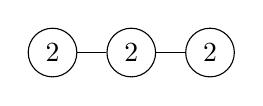
\begin{tikzpicture}[node/.style={circle, draw}]
        \node at (-1, 0) [node] (A) {$2$};
        \node at (0, 0) [node] (B) {$2$};
        \node at (1, 0) [node] (C) {$2$};
        \draw (A) -- (B) -- (C);
    \end{tikzpicture}
    \caption{Beispielgraph mit Knotengewichten\label{fig:graph}}
\end{figure}

